\chapter{Ranqueamento de \textit{Issues} no SPB}
\label{est}
\section{O Portal do Software Público Brasileiro}
\label{est:sof}
O portal do Software Público Brasileiro (SPB) é um espaço virtual, criado em 12 de abril de 2007, que agrega um conjunto de softwares desenvolvidos nas áreas de saúde, educação, saneamento, gestão de TI, Geoprocessamento, entre outras. Os serviços do SPB são acessados não só no Brasil, mas também por outros países, como por exemplo: Uruguai, Argentina, Portugal, Venezuela, Chile e Paraguai. A politica de compartilhamento de software resulta em uma gestão mais racionalizada de recursos e gastos em Tecnologia da Informação por parte da Administração Pública Federal. Isso possibilita também, a ampliação de parcerias e reforço da politica de software livre no setor público~\cite{spb}.

O novo Portal do Software Público Brasileiro é composto de:

\begin{itemize}
    \item Lista de discussão (Mailman).
    \item Plataforma de redes sociais com blog, e-Portifólios, RSS, discussão 
    temática, agenda de eventos, galeria de imagens, e demais funcionalidades de um CMS (Noosfero).
    \item Sistema de controle de versão, repositório de código-fonte e ambiente 
    desenvolvimento colaborativo (GitLab).
    \item Autenticação única, busca e integração de ferramentas a fim de tornar 
    a navegação intuitiva e transparente entre as diversas ferramentas que compõem 
    o novo Portal (Colab).
\end{itemize}

Este ambiente possui uma arquitetura de sete máquinas com funções distintas que são fundamentais para que estes serviços sejam fornecidos. Um destes ambientes, chamado de \textit{reverse proxy}, ou proxy reverso,  trata todas as requisições HTTP e as direciona para uma segunda máquina onde as requisições são distribuidas para os ambientes que fornecem o serviço solicitado~\cite{spbdocs}. A Figura~\ref{fig:arquitetura} mostra como estes ambientes se comunicam e como são distribuídos os serviços em cada uma das máquinas.
\newpage
\begin{figure}[!h]
    \centering
        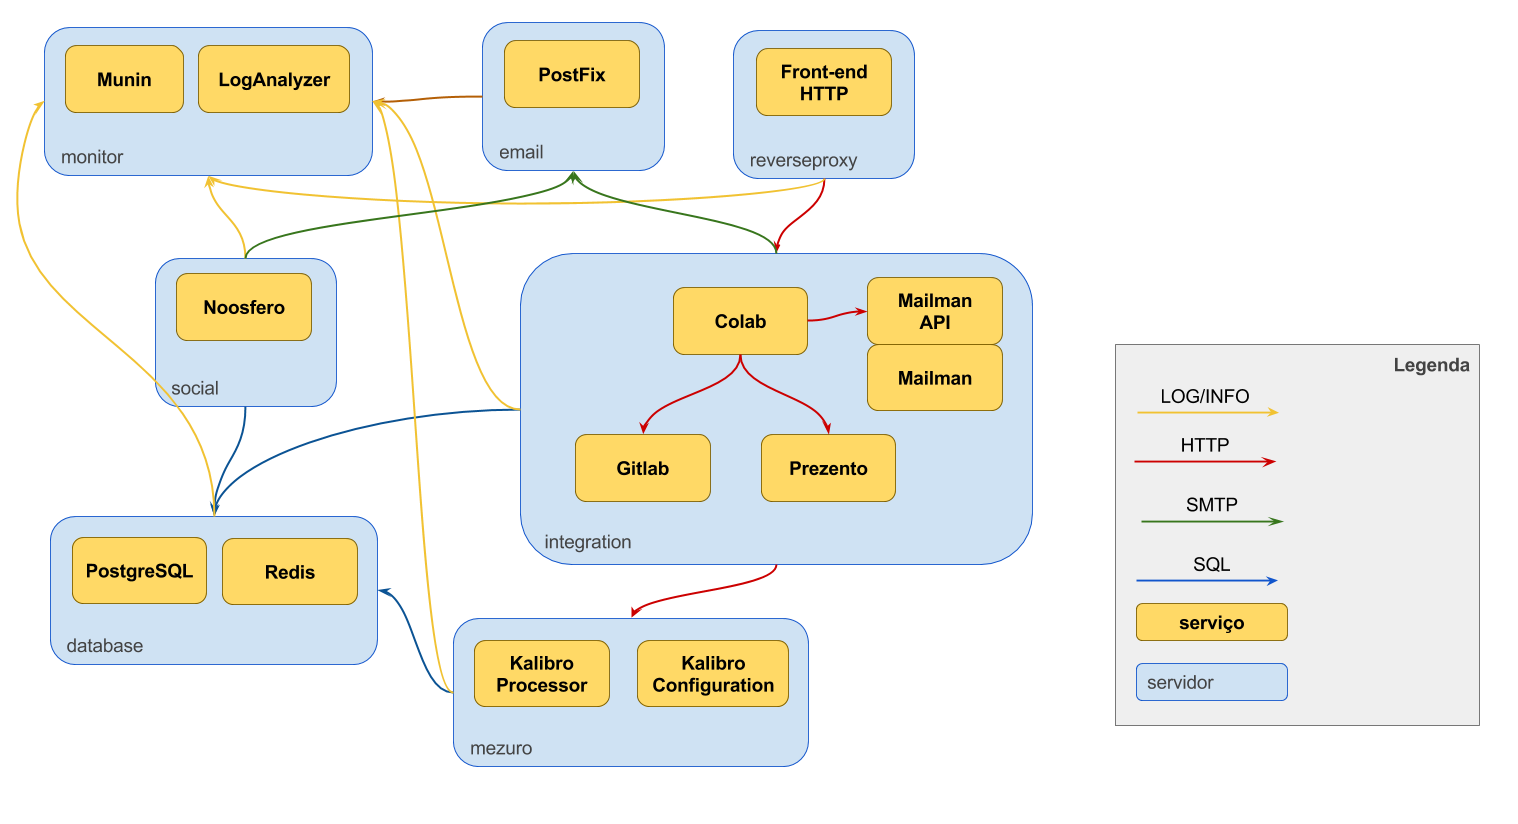
\includegraphics[keepaspectratio=true,scale=0.3]{figuras/arquitetura.eps}
    \caption{Diagrama da Arquitetura do SPB, extraída de~\cite{spbdocs}}
    \label{fig:arquitetura}
\end{figure}

\begin{itemize}
    \item \textbf{Reverse Proxy:} Proxy reverso.
    \item \textbf{Integration:} Segundo proxy reverso, repositorio git, listas de email e \textit{backend} final de e-mail.
    \item \textbf{Email:} Relay de e-mail.
    \item \textbf{Social:} Servidor da rede social Noosfero.
    \item \textbf{Database:} Servidor de banco de dados PostgreSQL
    \item \textbf{Mezuro:} Servidor de análise de código Mezuro.
    \item \textbf{Monitor:} Monitoramento e informações dos outros serviços.
\end{itemize}

\section{Organização do Trabalho No SPB}
\label{est:sof}

O Software Público Brasileiro foi desenvolvido com base no \textit{Scrum}. O \textit{Scrum} é um método para gerenciar o desenvolvimento e manutenção de produtos, criado em meados da década de 1990 por \cite{scrum}. O \textit{Scrum} é flexível o suficiente para permitir que outros processos, métodos ou práticas possam ser empregados conjuntamente com ele.

Como métodos de desenvolvimento do SPB, foram utilizadas adaptações do \textit{Scrum} e do XP, além de práticas de \textit{DevOps}, mantendo contudo os valores prescritos no manifesto ágil. Sendo assim, o projeto foi dividido em três níveis, o nível operacional, o nível tático e o  nível estratégico. Dentro do nível estratégico são definidas as metas estratégicas de cada \textit{release}, o período de duração, e as épicas de negocio. Dentro do nível tático é onde existe a interação entre os responsáveis pelo projeto na UnB e os representantes do MPOG, neste nível que são definidos quais as \textit{features} que deverão ser implementadas na próxima \textit{release} e a priorização das mesmas. A medida que desce-se o nível a partir das metas estratégicas e do planejamento tático e nos aproximamos do nível operacional, o grau de granularidade aumenta até chegar a micro atividades, ou seja ao nível de tarefas diárias executadas pelos desenvolvedores do projeto. Podemos ver essa divisão ocorrendo nas Figuras~\ref{fig:spb-layers} e~\ref{fig:epics-wiki} abaixo, que mostram como essa quebra é feita e como isso acontece na \textit{Wiki} do projeto.

\begin{figure}[!h]
    \centering
        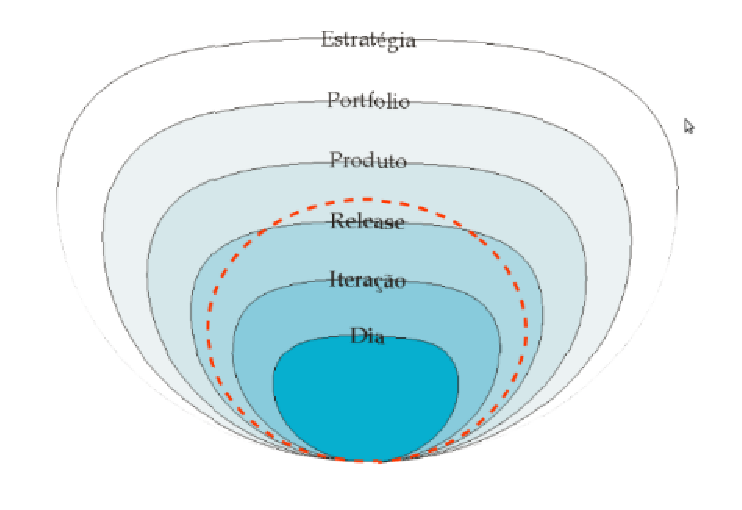
\includegraphics[keepaspectratio=true,scale=0.7]{figuras/spb-layers.eps}
    \caption{Diagrama Dos Níveis de Projeto do SPB, extraído de \textit{SPB - RIO Info}}
    \label{fig:spb-layers}
\end{figure}

\begin{figure}[!h]
    \centering
        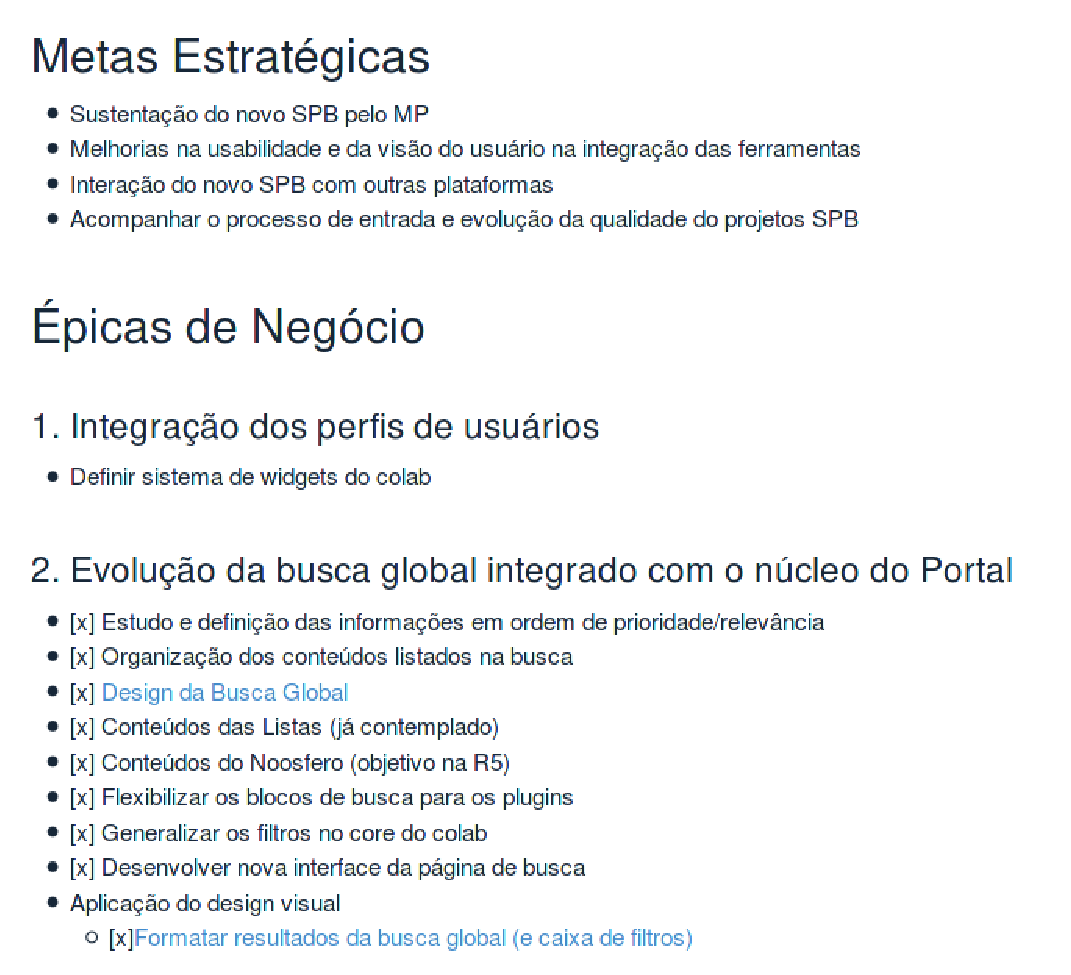
\includegraphics[keepaspectratio=true,scale=0.5]{figuras/wiki.eps}
    \caption{Wiki do SPB com as Métas de Estratégicas e Épicas de Negócio}
    \label{fig:epics-wiki}
\end{figure}

Já dentro do nível operacional existem as histórias de usuário e as atividades. Dentro do SPB, as histórias de usuário são tratadas como \textit{milestones}  e as atividades como \textit{issues} do Gitlab. Dentro de uma \textit{sprint} cada time escolhe uma ou mais  histórias, do \textit{backlog} da \textit{release}, e realiza a divisão de suas atividades entre seus membros. A utilização da ferramenta Gitlab permite que as atividades possam ser comentadas e acompanhadas pelos usuários, facilitando, desta forma, o acompanhamento do projeto tanto por parte do Ministério do Planejamento Orçamento e Gestão e dos desenvolvedores. As imagens~\ref{fig:milestone} e~\ref{fig:issue} abaixo mostram a estrutura de uma história e de uma atividade.

\begin{figure}[!h]
    \centering
        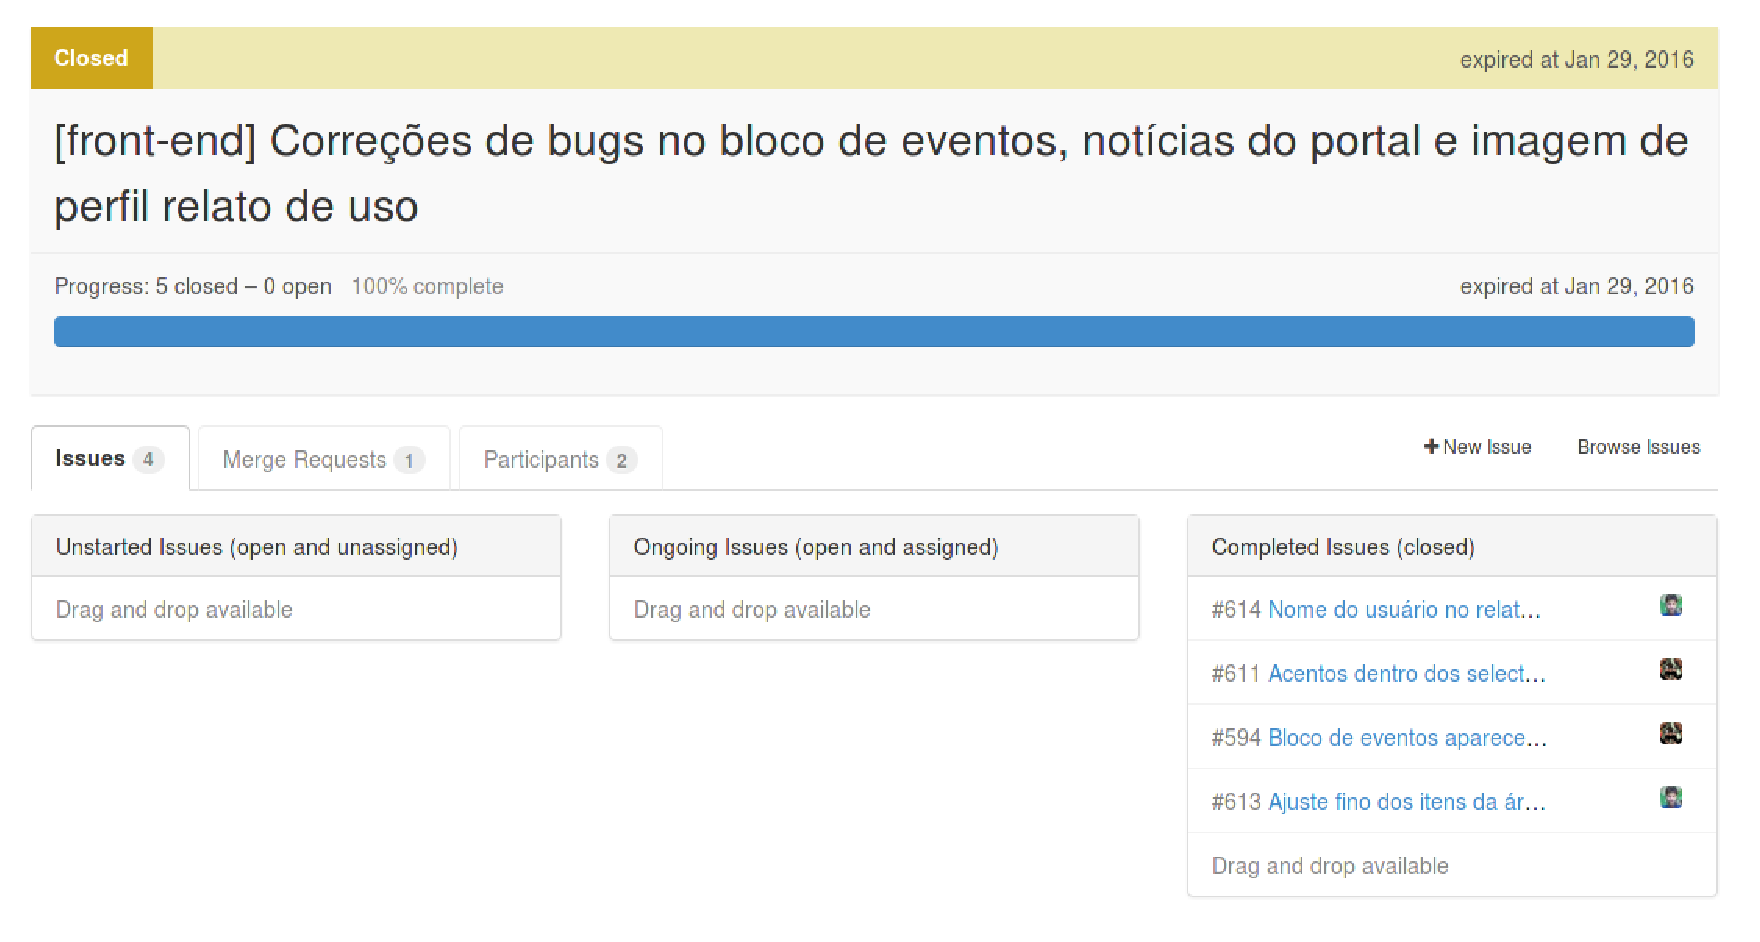
\includegraphics[keepaspectratio=true,scale=0.5]{figuras/milestone.eps}
    \caption{Estrutura de um \textit{Milestone} no SPB}
    \label{fig:milestone}
\end{figure}


\begin{figure}[!h]
    \centering
        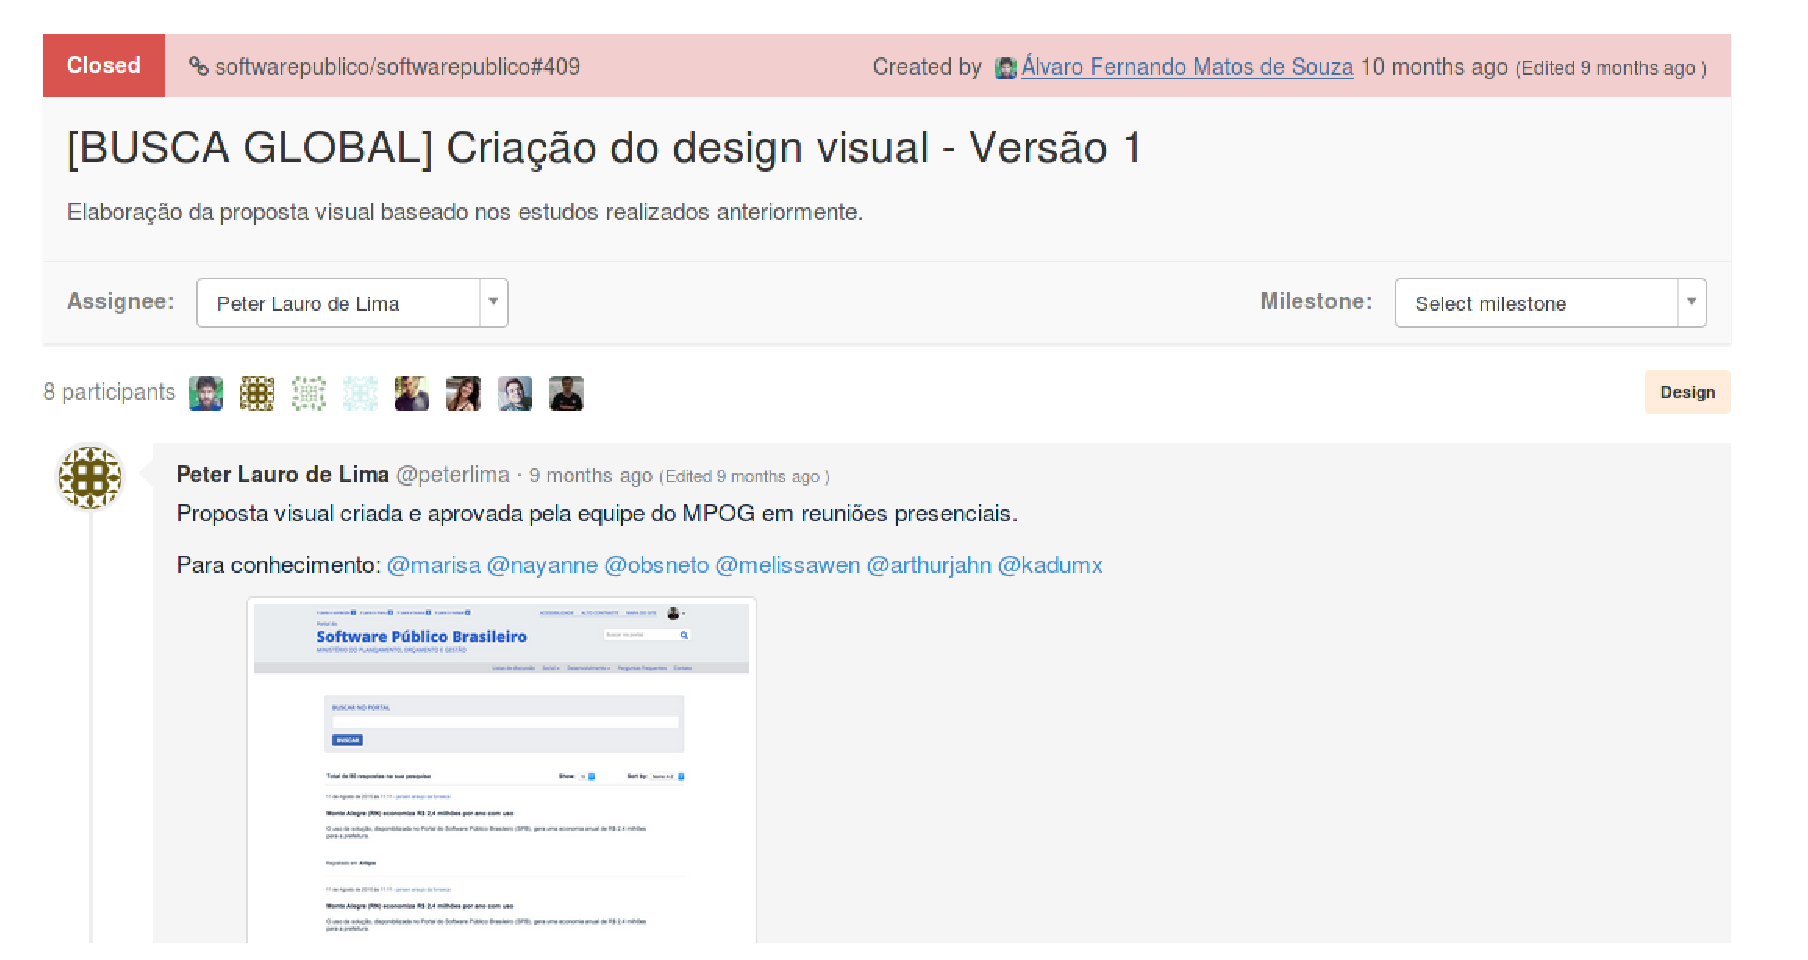
\includegraphics[keepaspectratio=true,scale=0.5]{figuras/issue.eps}
    \caption{Estrutura de uma \textit{Issue} no SPB}
    \label{fig:issue}
\end{figure}

A escolha do SPB como um caso piloto foi estratégica, visto que é um projeto de domínio público e utilizando o Gitlab, é possível exportar informações de desenvolvedores, atividades, histórias e épicas, além disto é possível extrair informações especificas relacionadas ao código fonte do projeto. Sem este tipo de acesso a informação seria praticamente impossível a execução deste experimento. Outro fator determinante é a forma com o que o SPB concentra o planejamento de \textit{release} dentro da repositório, o permite com que a relação entre as atividades seja evidenciada mais facilmente.

\section{Ranqueamento de Páginas no SPB}
\label{est:ran}

Essa sessão apresenta como o algoritmo de ranqueamento de páginas descrito no apêndice~\ref{ape:cod} foi aplicado ao Software Público Brasileiro de forma a extrair a relevância das \textit{issues} das \textit{releases} 4 e 5. Como foi dita na sessão~\ref{est:sof}, a escolha deste projeto para o estudo de caso foi estratégica de forma a facilitar a execução deste experimento, já que o SPB possui  estrutura e condições favoráveis a isso.

\subsection{Vértices e Arestas}
\label{est:ran:ver}

Como foi visto na Seção~\ref{ref:cen:pag} a utilização do algoritmo de ranqueamento de páginas depende que inicialmente exista um grafo direcionado.\footnote{Um grafo direcionado, ou dígrafo, $D$ consiste de um conjunto finito de elementos não vazios $V(D)$ chamados de vértices e um conjunto finito $A(D)$ de pares ordenados de vértices distintos chamados arcos. Desta forma, $V(D)$ é chamado de conjunto de vértices e $A(D)$ o conjunto de arcos de $D$~\cite{bang}.}

Para que um grafo do SPB fosse gerado, foi utilizada a API do Gitlab juntamente com um \textit{script Python} para que todas as \textit{issues}, \textit{milestones} e comentários fosse exportado em formato JSON, isto pode ser visto nos métodos \textit{get\_repo\_issues} e~\textit{get\_repo\_milestones} do apêndice~\ref{ape:cod}. Como foi dito, o algoritmo de ranqueamento de páginas precisa de um dígrafo para ser executado, uma das adaptações deste \textit{script} é que em alguns casos os grafos gerados não eram direcionados, e por isto, estes grafos tiveram que ser convertidos em grafos direcionados substituindo cada um dos arcos ou arestas por um arco de entrada e um de saída, este processo pode ser visto nas Figuras~\ref{fig:undirected} e~\ref{fig:directed}.

\begin{figure}[!h]
    \centering
        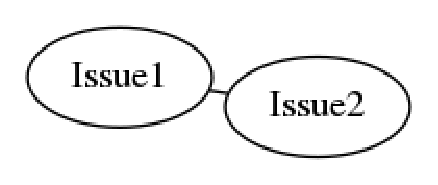
\includegraphics[keepaspectratio=true,scale=0.5]{figuras/undirected.eps}
    \caption{\textit{Issues} antes da conversão dos arcos}
    \label{fig:undirected}
\end{figure}

\begin{figure}[!h]
    \centering
        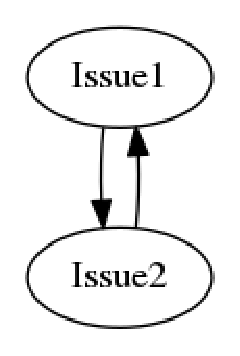
\includegraphics[keepaspectratio=true,scale=0.5]{figuras/directed.eps}
    \caption{\textit{Issues} depois da conversão dos arcos}
    \label{fig:directed}
\end{figure}

\subsubsection{Issues}
\label{est:ran:iss}

Como o foco do estudo é analisar a relevância das \textit{issues}, o dígrafo foi gerado com base nelas com o método \textit{gen\_raph} no apêndice~\ref{ape:cod}. Dentro do grafo, cada \textit{issue} foi tratada como um vértice, e as arestas eram formadas a medida que uma \textit{issue} era marcada, através de comentários ou eventos, dentro de outra. A Figura~\ref{fig:issue-comment} exemplifica esse processo.

\begin{figure}[!h]
    \centering
        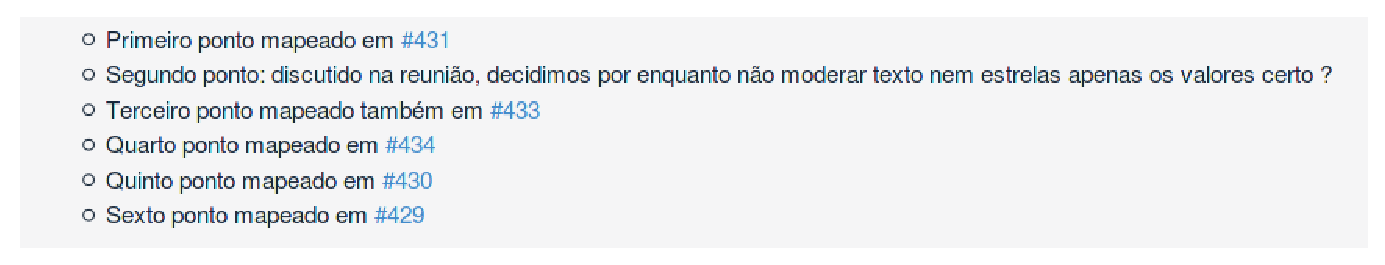
\includegraphics[keepaspectratio=true,scale=0.7]{figuras/issue-comment.eps}
    \caption{Exemplo de comentário com marcação de \textit{issue}}
    \label{fig:issue-comment}
\end{figure}

Para a realização deste processo foram analisados os comentários de todas as 879 \textit{issues} no repositório do SPB. O dígrafo gerado por esse processo, foi então utilizado para a aplicação do algoritmo de ranqueamento de páginas, a Figura ~\ref{fig:issue-graph} demonstra como esse grafo se apresenta.

\begin{figure}[!h]
    \centering
        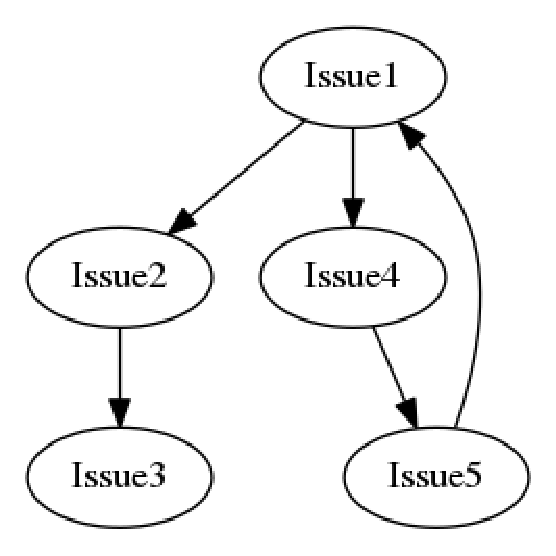
\includegraphics[keepaspectratio=true,scale=0.5]{figuras/issue-graph.eps}
    \caption{Demonstração de grafo das \textit{issues}}
    \label{fig:issue-graph}
\end{figure}


\subsubsection{\textit{Milestones}}
\label{est:ran:mil}

Dentro do projeto SPB, um \textit{milestone} é uma história com um conjunto de \textit{issues} associadas. Para que fosse possível uma maior aproximação com o ranqueamento de páginas considerou-se que todas as \textit{issues} dentro de um \textit{milestones} estão interligadas, de forma que elas formem um grafo completo\footnote{Um grafo $G$ é considerado como completo se cada par de vértices distintos em $G$ são adjacentes~\cite{bang}.}, essa abstração pode ser vista na Figura~\ref{fig:milestone-graph}.

\begin{figure}[!h]
    \centering
        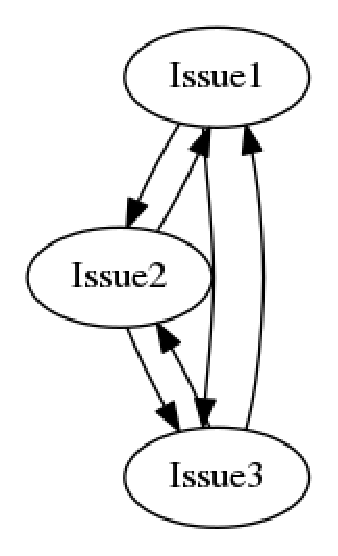
\includegraphics[keepaspectratio=true,scale=0.5]{figuras/milestone-graph.eps}
    \caption{Demonstração de grafo das \textit{issues} em um mesmo  \textit{milestones}}
    \label{fig:milestone-graph}
\end{figure}

\newpage
\section{Resultados}
\label{est:res}

Utilizando-se das abstrações descritas na Seção \ref{est:ran} foi possível gerar um grafo representando as \textit{issues} do SPB, esta execução pode ser vista no método \textit{run\_pagerank} disponível no apêndice~\ref{ape:cod}. Este grafo apresenta as \textit{issues} mais altamente conectadas no centro e as menos conectadas nas bordas. Na Figura \ref{fig:graph}, é possível perceber que a grande maioria das \textit{issues} tem poucas conexões, ou seja, possuem poucos comentários de marcação, além disto, em alguns casos estas \textit{issues} não estavam associadas a nenhum \textit{milestone}. Esse comportamento pode denotar um baixo índice de comunicação entre a equipe de desenvolvimento e os \textit{stakeholders} no inicio do projeto.

\begin{figure}[!h]
    \centering
        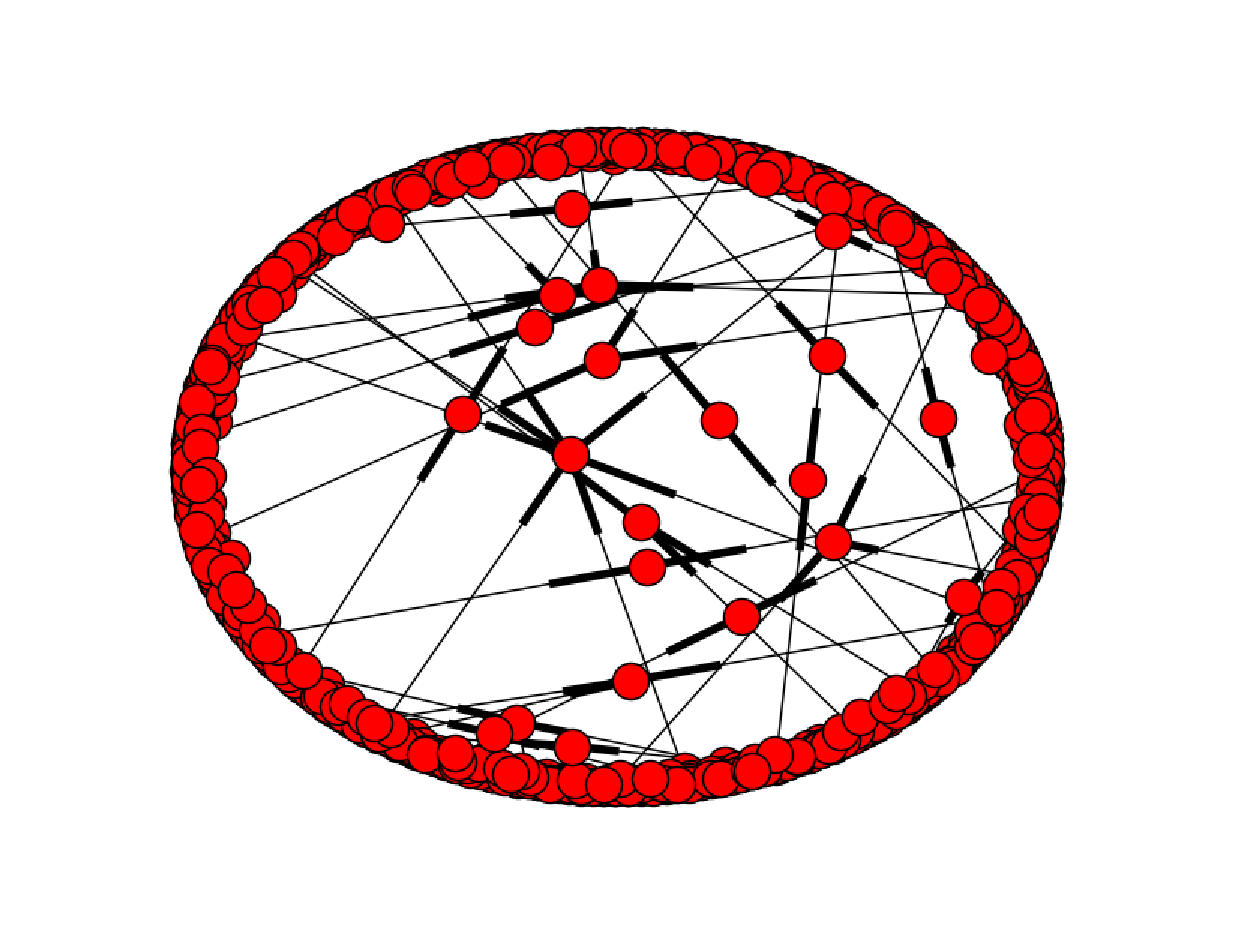
\includegraphics[keepaspectratio=true,scale=0.5]{figuras/graph.eps}
    \caption{Grafo das \textit{issues} do SPB}
    \label{fig:graph}
\end{figure}

A partir do grafo representado na Figura \ref{fig:graph}, foi executado o algoritmo de ranqueamento de páginas, o algoritmo utilizado foi o \textit{Page Ranking}, discutido na Seção \ref{ref:ran}. Para permitir a execução do algoritmo, foram utilizadas as abstrações para \textit{issues} e \textit{milestones} discutidas nas seções \ref{est:ran:iss} e \ref{est:ran:mil}. Após a execução, o algoritmo exporta as \textit{issues} associadas a um valor numérico, de forma que, quanto maior o valor associado a uma \textit{issue}, maior o seu ranque relativo. No SPB, as dez \textit{issues} com o maior ranque relativo estão apresentadas na tabela \ref{tab:pagerank}. 

\begin{table}[h]
    \begin{tabularx}{\textwidth}{|X|r|}
        \toprule
    	\textbf{Issues} & \textbf{Pagerank} \\
    	\hline	
            \midrule
            Moderação do valor dos recursos economizados do relato de uso & 0.0059332219490603475 \\ \hline
            Configurar o \textit{NGINX} para servir os dados do \textit{syslog} & 0.003453026773943251 \\ \hline
            Exibir mensagem de erro próxima ao campo instituição no relato de uso &  0.003453026773943251 \\\hline
            Subir o Gitlab 8.5 usando o pacote feito. & 0.003453026773943251 \\\hline
            Melhora da busca global & 0.003453026773943251 \\\hline
            Tela branca em Editar blocos laterais de comunidade & 0.003453026773943251 \\\hline
            Importar as notícias wiki do portal &  0.0030396609114237347 \\\hline
            Cadastro de usuário quebrado (username: boscojr) & 0.002626295048904218 \\\hline
            Adicionar e-mail do usuário na Tela de processar solicitação de Entrar na comunidade. & 0.002626295048904218 \\\hline
            Retirar pergunta por SISP na criação de uma nova instituição? & 0.002626295048904218 \\\hline
            \bottomrule
    \end{tabularx}
    \label{tab:pagerank}
    \caption{As dez \textit{issues} melhor ranqueadas do Software Publico Brasileiro}
\end{table}

Com base nas \textit{issues} melhores ranqueadas, foi possível perceber que alguns termos aparecem com maior frequência, são eles: \textbf{Relato de Uso}, \textbf{Busca Global}, \textbf{Gitlab} e \textbf{SISP}. Outras das \textit{issues} que aparecem com o ranque alto, estão ligadas a atividades de manutenção, sejam elas: correção de \textit{bugs}, melhorias de \textit{front-end} e infraestrutura. Desta forma, aparentemente, as \textit{features} de implementação do relato de uso, da busca global, atualização do Gitlab e algumas das correções de \textit{bugs} foram consideradas de maior importância do que aquelas que apresentaram grau de relevância menor.

Através destes dados foi possível realizar uma comparação manual com o planejamento das \textit{releases} 4 e 5 do SPB. Essa comparação foi feita através da comparação dos termos das \textit{issues} mais bem ranqueadas com o \textit{backlog} presente na \textit{Wiki}. Para essas \textit{releases} algumas da \textit{features} prioritárias são: a implementação do relato de uso de software, evolução da busca global e melhorias gerais, termos comuns aos de muitas das \textit{issues} com ranque alto.  Já o termo Gitlab aparece com uma alta relevância devido ao grande esforço dedicado a atualização da plataforma durante a fase de finalização do projeto, mas que devido a finalização antecipada da parceria UnB com o MPOG a nova plataforma foi disponibilizada porém não pôde ser integrada. As Figuras \ref{fig:relato} e \ref{fig:busca} mostram como essas épicas de negocio estão presentes na \textit{Wiki} do projeto e como foram organizadas.

\begin{figure}[!h]
    \centering
        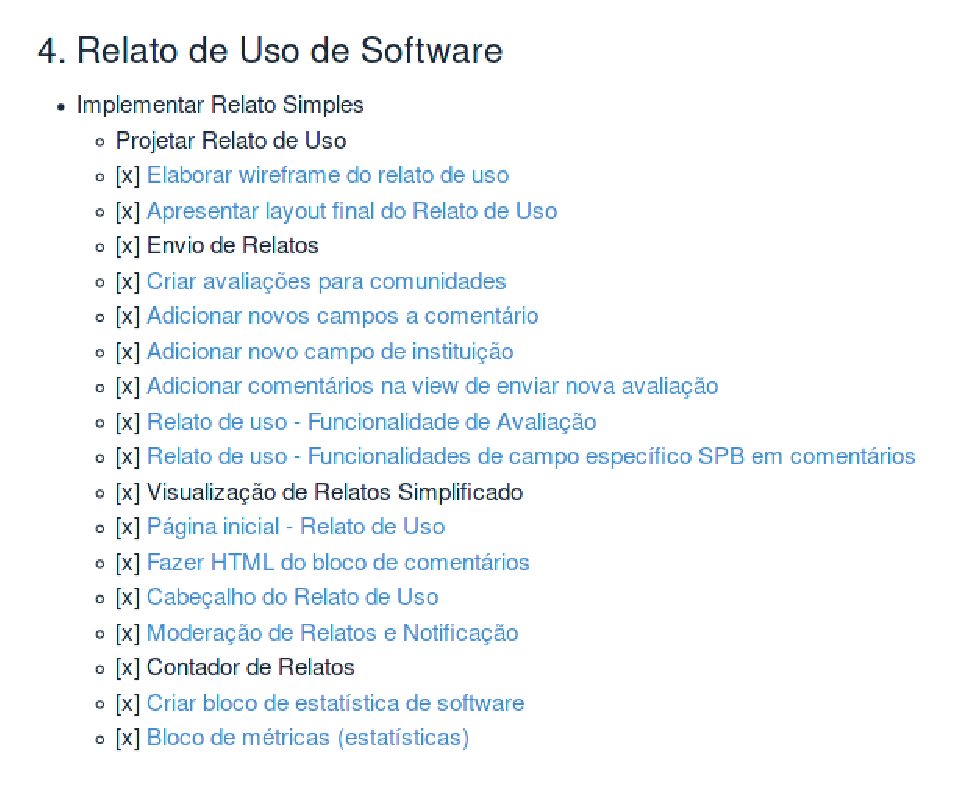
\includegraphics[keepaspectratio=true,scale=0.5]{figuras/relato.eps}
    \caption{Épica de Negocio de Relato de Uso}
    \label{fig:relato}
\end{figure}

\begin{figure}[!h]
    \centering
        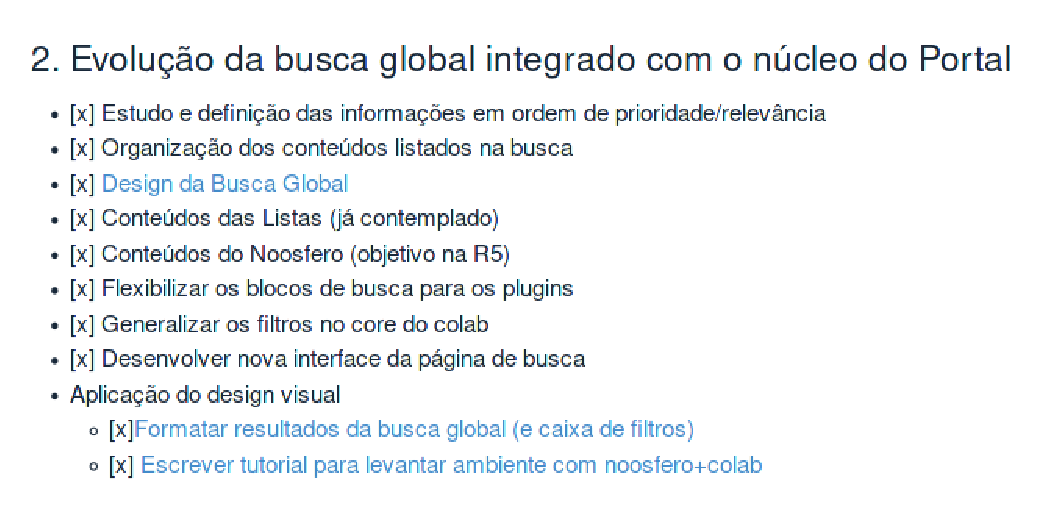
\includegraphics[keepaspectratio=true,scale=0.5]{figuras/busca.eps}
    \caption{Épica de Negocio da Melhoria da Busca Global}
    \label{fig:busca}
\end{figure}

\newpage
Outro grande conjunto de \textit{issues} com alto ranque estão ligadas a épica de negocio de melhorias gerais. Indicando que durante parte do desenvolvimento houveram muitas interações entre os \textit{product owners} do MPOG e a equipe de desenvolvedores da UnB e os \textit{seniors} do projeto.

No SPB, as \textit{issues} bem ranqueadas possuem uma correlação de termos com as \textit{features} que demandaram grande parte do esforço do projeto nas \textit{releases} 4 e 5. Desta forma, caso o projeto ainda estivesse em atividade possivelmente as próximas \textit{sprints} poderiam utilizar da aplicação deste ranqueamento para criar um possível \textit{roadmap} e assim validar a solução proposta.

\section{Considerações Finais do Capítulo}
Neste capítulo foram apresentadas as técnicas utilizadas para a busca, mineração e análise utilizadas para o ranqueamento das \textit{issues} do Software Público Brasileiro. Primeiramente foi apresentado o projeto escolhido para o exemplo de uso, depois foram apresentadas os métodos utilizados para a modelagem das \textit{issues} em um grafo direcionado e em seguida foi explicado como o algoritmo de ranqueamento de páginas foi aplicado, gerando assim resultados preliminares para este trabalho. No próximo capítulo são apresentadas as conclusões preliminares, os trabalhos futuros para a segunda etapa deste trabalho e um cronograma de atividades.
